\documentclass[12pt]{article}
\usepackage[margin=0.5in]{geometry}
\usepackage{amsmath}
\usepackage{amsfonts}
\usepackage{tikz}
\usetikzlibrary{positioning, calc, shapes.geometric, shapes, shapes.multipart, arrows.meta, arrows, decorations.markings, external, trees}

\tikzstyle{Arrow} = [
    thick,
    decoration={
        markings,
		mark=at position 1 with {
            \arrow[thick]{latex}
		}
	},
	shorten >= 3pt, preaction = {decorate}
]


\begin{document}

\title{Identification and Estimation of Causal Effects}
\maketitle

Resources:
\begin{itemize}
    \item What is the difference between $a^*$, $a$, and $a^{+g}$?
    \item E-mail Jessica SWIG; document fast food; GitHub discussion; StackExchange posts.
    \item Why in time-varying settings, sums translate to prediction and plug-in?
    \item $E[Y^g|l,a^{+g}]f(a^{+g}|a)$: what if $A$ is continuous? Just multiply?
\end{itemize}

%%%%%%%%%%%%%%%%%%%%%%%%%%%%%%%%%%
\section{Time-invariant Exposures}
%%%%%%%%%%%%%%%%%%%%%%%%%%%%%%%%%%

\subsection{Deterministic Treatment Regimes}
The rule for assigning treatment does so with probability 1.

\subsubsection*{Deterministic Static Treatment Regimes}
The rule for assigning treatment does not depend on past treatment or covariates.

\begin{figure}[h]
\centering
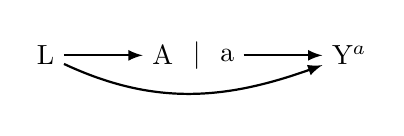
\begin{tikzpicture}[
array/.style={
    rectangle split,
	rectangle split parts = 3,
	rectangle split horizontal,
    minimum height = 2em
    }
]

\node (1) {L};
\node [array, right = of 1] (2) {
    {A}
    \nodepart{two}{$|$}
    \nodepart{three}{a}
};
\node [right = of 2] (3) {Y$^a$};

\draw[Arrow, thick] (1.east) -- (2.west);
\draw[Arrow, thick] (1) to [out=335, in=200] (3);

\draw[Arrow, thick] (2.east) -- (3.west);

\end{tikzpicture}
\caption{A SWIG representing a static treatment regime.}
\label{fig:swig_det_stat_inv}
\end{figure}

The joint density is:

\begin{equation}
    f(y,l,a) = f(y|l,a) f(a|l) f(l).
\end{equation}

After intervening on the exposure $A$, we have:

\begin{equation}
    f^G(y,l) = f(y|l,\textcolor{red}{a}) f(l).
\end{equation}

Thus, the expected value of the outcome $Y$ is:

\begin{align}
    \mathbb{E}^G \left[ Y \right] &= \sum_y y f^G(y) \\
    &= \sum_y y \sum_l f^G(y,l) \\
    &= \sum_y \sum_l y f(y|l,\textcolor{red}{a}) f(l) \\
    &= \sum_l \mathbb{E} \left[ Y|A=\textcolor{red}{a},L=l\right] f(L=l).
\end{align}

\paragraph{Algorithm}

\subsubsection*{Deterministic Dynamic Treatment Regimes}
The rule for assigning treatment depends on past treatment or covariates.

\begin{figure}[h]
\centering
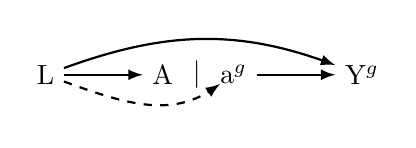
\begin{tikzpicture}[
array/.style={
    rectangle split,
	rectangle split parts = 3,
	rectangle split horizontal,
    minimum height = 2em
    }
]

\node (1) {L};
\node [array, right = of 1] (2) {
    {A}
    \nodepart{two}{$|$}
    \nodepart{three}{a$^g$}
};
\node [right = of 2] (3) {Y$^g$};

\draw[Arrow, thick] (1.east) -- (2.west);
\draw[Arrow, dashed] (1) to [out=340, in=215] (2.three);
\draw[Arrow, thick] (1) to [out=20, in=160] (3);

\draw[Arrow, thick] (2.east) -- (3.west);

\end{tikzpicture}
\caption{A SWIG representing a dynamic treatment regime.}
\label{fig:swig_det_dyn_inv}
\end{figure}

The joint density is:

\begin{equation}
    f(y,l,a,a^g) = f(y|l,a^g) f(a^g|l) f(a|l) f(l).
\end{equation}

\textcolor{red}{Does the term $f(a|l)$ \textit{go away} because we are setting the exposure $A$ to $a$, or is it incorporated with $f(l)$ into $f(a,l)$?}

After intervening on the exposure $A$, we have:

\begin{equation}
    f^G(y,l,a^g) = f(y|l,\textcolor{red}{a^g}) f(\textcolor{red}{a^g}|l) f(l).
\end{equation}

Thus, the expected value of the outcome $Y$ is:

\begin{align}
    \mathbb{E}^G \left[ Y \right] &= \sum_y y f^G(y) \\
    &= \sum_y y \sum_l \sum_{a^g} f^G(y,l,\textcolor{red}{a^g}) \\
    &= \sum_y \sum_l \sum_{a^g} y f(y|l,\textcolor{red}{a^g}) f(\textcolor{red}{a^g}|l) f(l) \\
    &= \sum_l \sum_{a^g} \mathbb{E} \left[ Y|A=\textcolor{red}{a^g},L=l\right] f(\textcolor{red}{a^g}|L=l) f(L=l).
\end{align}

\paragraph{Algorithm}

\subsubsection*{Deterministic Natural Treatment Regimes}
The rule for assigning treatment depends on its natural value.

\begin{figure}[h]
\centering
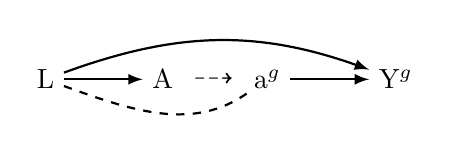
\begin{tikzpicture}[
array/.style={
    rectangle split,
	rectangle split parts = 3,
	rectangle split horizontal,
    minimum height = 2em
    }
]

\node (1) {L};
\node [array, right = of 1] (2) {
    {A}
    \nodepart{two}{$\dashrightarrow$}
    \nodepart{three}{a$^g$}
};
\node [right = of 2] (3) {Y$^g$};

\draw[Arrow, thick] (1.east) -- (2.west);
\draw[Arrow, dashed] (1) to [out=340, in=215] (2.three);
\draw[Arrow, thick] (1) to [out=20, in=160] (3);

\draw[Arrow, thick] (2.east) -- (3.west);

\end{tikzpicture}
\caption{A SWIG representing a natural treatment regime.}
\label{fig:swig_det_nat_inv}
\end{figure}

The joint density is:

\begin{equation}
    f(y,l,a,a^g) = f(y|l,a^g) f(a^g|l,a) f(a|l) f(l).
\end{equation}

\textcolor{red}{Does the term $f(a|l)$ \textit{go away} because we are setting the exposure $A$ to $a$, or is it incorporated with $f(l)$ into $f(a,l)$? If it is removed, where does the summation over $a$ come from?}

After intervening on the exposure $A$, we have:

\begin{equation}
    f^G(y,l,a,a^g) = f(y|l,\textcolor{red}{a^g}) f(\textcolor{red}{a^g}|l,a) f(a|l) f(l).
\end{equation}

Thus, the expected value of the outcome $Y$ is:

\begin{align}
    \mathbb{E}^G \left[ Y \right] &= \sum_y y f^G(y) \\
    &= \sum_y y \sum_l \sum_a \sum_{a^g} f^G(y,l,a,\textcolor{red}{a^g}) \\
    &= \sum_y \sum_l \sum_a \sum_{a^g} y f(y|l,\textcolor{red}{a^g}) f(\textcolor{red}{a^g}|l,a) f(a|l) f(l) \\
    &= \sum_l \sum_a \sum_{a^g} \mathbb{E} \left[ Y|A=\textcolor{red}{a^g},L=l\right] f(\textcolor{red}{a^g}|a,L=l) f(a|l) f(L=l).
\end{align}

\paragraph{Algorithm}

\subsubsection*{Modified Treatment Policies}

\subsection{Random Treatment Regimes}
The rule for assigning treatment does so with probability between 0 and 1.

%%%%%%%%%%%%%%%%%%%%%%%%%%%%%%%%
\section{Time-varying Exposures}
%%%%%%%%%%%%%%%%%%%%%%%%%%%%%%%%

\subsection{Deterministic Treatment Regimes}
The rule for assigning treatment does so with probability 1.

\subsubsection*{Deterministic Static Treatment Regimes}
The rule for assigning treatment does not depend on past treatment or covariates.

If $f^{\text{int}} (a_k | \bar{a}_{k-1}, \bar{D}_k=0)$ is either 0 or 1 for each $\bar{a}_k$ and for $k = 0,\dots,K$. In particular, given the regime $g = (g_0,\dots,g_K)$, $f^{\text{int}} (a_k | \bar{a}_{k-1}^g, \bar{D}_k=0) = 1$ if $a_k = a_k^g$, and 0 otherwise, with $a_s^g = g_s(\bar{a}_{s-1}^g)$.

\begin{figure}[h]
\centering
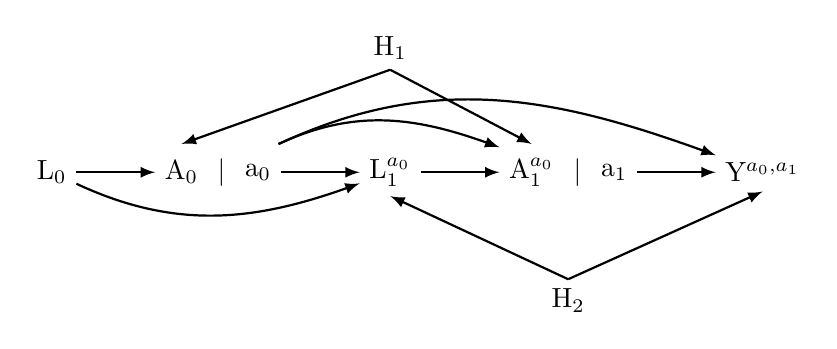
\begin{tikzpicture}[
array/.style={
    rectangle split,
	rectangle split parts = 3,
	rectangle split horizontal,
    minimum height = 2em
    }
]

\node (1) {L$_0$};
\node [array, right = of 1] (2) {
    {A$_0$}
    \nodepart{two}{$|$}
    \nodepart{three}{a$_0$}
};
\node [right = of 2] (3) {L$_1^{a_{0}}$};
\node [array, right = of 3] (4) {
 	{A$_1^{a_{0}}$}
    \nodepart{two}{$|$}
    \nodepart{three}{a$_1$}
};
\node [right = of 4] (5) {Y$^{a_0, a_1}$};
\node [right = of 2, above = of 3] (6) {H$_1$};
\node [right = of 3, below = of 4] (7) {H$_2$};

\draw[Arrow, thick] (6.south) -- (2.one north);
\draw[Arrow, thick] (6.south) -- (4.one north);
\draw[Arrow, thick] (7.north) -- (3.south);
\draw[Arrow, thick] (7.north) -- (5.south);

\draw[Arrow, thick] (1.east) -- (2.west);
\draw[Arrow, thick] (1) to [out=335, in=200] (3);

\draw[Arrow, thick] (2.east) -- (3.west);
\draw[Arrow, thick] (2) to [out=25, in=160] (4);
\draw[Arrow, thick] (2) to [out=25, in=160] (5);

\draw[Arrow, thick] (3.east) -- (4.west);

\draw[Arrow, thick] (4.east) -- (5.west);

\end{tikzpicture}
\caption{A SWIG representing a static treatment regime.}
\label{fig:swig_det_stat}
\end{figure}

\subsubsection*{Deterministic Dynamic Treatment Regimes}
The rule for assigning treatment depends on past treatment or covariates.

If $f^{\text{int}} (a_k | \bar{l}_k, \bar{a}_{k-1}, \bar{D}_k=0)$ is either 0 or 1 for each $(\bar{a}_k, \bar{l}_k)$ and for $k = 0,\dots,K$. In particular, given the regime $g = (g_0,\dots,g_K)$, $f^{\text{int}} (a_k | \bar{l}_k, \bar{a}_{k-1}^g, \bar{D}_k=0) = 1$ if $a_k = a_k^g$, and 0 otherwise, with $a_s^g = g_s(\bar{l}_s, \bar{a}_{s-1}^g)$.

\subsubsection*{Deterministic Natural Treatment Regimes}
The rule for assigning treatment depends on its natural value.

\begin{figure}[h]
\centering
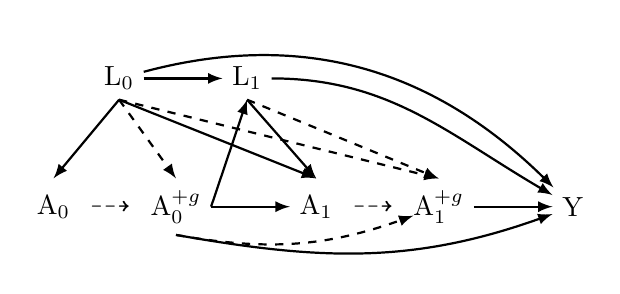
\begin{tikzpicture}[
array/.style={
    rectangle split,
	rectangle split parts = 3,
	rectangle split horizontal,
    minimum height = 2em
    }
]

\node (1) {L$_0$};
\node [array, below = of 1] (2) {
    {A$_0$}
    \nodepart{two}{$\dashrightarrow$}
    \nodepart{three}{A$_0^{+g}$}
};
\node [right = of 1] (3) {L$_1$};
\node [array, right = of 2] (4) {
 	{A$_1$}
    \nodepart{two}{$\dashrightarrow$}
    \nodepart{three}{A$_1^{+g}$}
};
\node [right = of 4] (5) {Y};

\draw[Arrow, thick] (1.south) -- (2.one north);
\draw[Arrow, dashed] (1.south) -- (2.three north);
\draw[Arrow, thick] (1.east) -- (3.west);
\draw[Arrow, thick] (1) to [out=15, in=135] (5);
\draw[Arrow, thick] (1.south) -- (4.one north);
\draw[Arrow, dashed] (1.south) -- (4.three north);

\draw[Arrow, thick] (2.three east) -- (3.south);
\draw[Arrow, thick] (2.three east) -- (4.one west);
\draw[Arrow, thick] (2.three south) to [out=350, in=200] (5);
\draw[Arrow, dashed] (2.three south) to [out=350, in=200] (4.three);

\draw[Arrow, thick] (3.south) -- (4.one north);
\draw[Arrow, dashed] (3.south) -- (4.three north);
\draw[Arrow, thick] (3.east) to [out=360, in=150] (5);

\draw[Arrow, thick] (4.east) -- (5.west);

\end{tikzpicture}
\caption{A SWIG representing a natural treatment regime.}
\label{fig:swig_det_nat}
\end{figure}

The joint density is:

\begin{align}
    f(y,l_0,l_1,a_0,a_0^g,a_1,a_1^g) = &f(y|l_0,l_1,a_0^g,a_1^g)\times\\
    &f(a_1^g|l_0,l_1,a_0^g,a_1)\times\\
    &f(a_1|l_0,l_1,a_0^g)\times\\
    &f(l_1|l_0,a_0^g)\times\\
    &f(a_0^g|l_0,a_0)\times\\
    &f(a_0|l_0) f(l_0).
\end{align}

\textcolor{red}{Do the terms $f(a_t|\bar{l},\bar{a}_{t-1}^g)$ \textit{go away} because we are setting the exposure $A_t$ to $a_t$, or are they incorporated somewhere? If they are removed, where do the summations over $a_t$ come from?}

After intervening on the exposure $A$, we have:

\begin{align}
    f(y,l_0,l_1,a_0,a_0^g,a_1,a_1^g) = &f(y|l_0,l_1,\textcolor{red}{a_0^g},\textcolor{red}{a_1^g)}\times\\
    &f(\textcolor{red}{a_1^g}|l_0,l_1,\textcolor{red}{a_0^g},a_1)\times\nonumber\\
    &f(a_1|l_0,l_1,\textcolor{red}{a_0^g})\times\nonumber\\
    &f(l_1|l_0,\textcolor{red}{a_0^g})\times\nonumber\\
    &f(\textcolor{red}{a_0^g}|l_0,a_0)\times\nonumber\\
    &f(a_0|l_0) f(l_0)\nonumber.
\end{align}

Thus, the expected value of the outcome $Y$ is:

\begin{align}
    \mathbb{E}^G \left[ Y \right] &= \sum_y y f^G(y) \\
    &= \sum_y y \sum_{l_0} \sum_{l_1} \sum_{a_0} \sum_{a_0^g} \sum_{a_1} \sum_{a_1^g} f^G(y,l_0,l_1,a_0,\textcolor{red}{a_0^g},a_1,\textcolor{red}{a_1^g}) \\
    &= \sum_{l_0} \sum_{l_1} \sum_{a_0} \sum_{a_0^g} \sum_{a_1} \sum_{a_1^g}
    \!\begin{aligned}[t]
        &\mathbb{E} \left[ Y|L_0=l_0,L_1=l_1,A_0=\textcolor{red}{a_0^g},A_1=\textcolor{red}{a_1^g}\right]\times\\
        &f(\textcolor{red}{a_1^g}|l_0,l_1,\textcolor{red}{a_0^g},a_1)\times\\
        &f(a_1|l_0,l_1,\textcolor{red}{a_0^g})\times\\
        &f(l_1|l_0,\textcolor{red}{a_0^g})\times\\
        &f(\textcolor{red}{a_0^g}|l_0,a_0)\times\\
        &f(a_0|l_0) f(l_0).
    \end{aligned}
\end{align}

More generally, when there are more than two time points, we have:

\begin{align}
    \mathbb{E}^G \left[ Y \right] &= \sum_y y f^G(y) \\
    &= \sum_y y \sum_{l_0} \sum_{l_1} \sum_{a_0} \sum_{a_0^g} \sum_{a_1} \sum_{a_1^g} f^G(y,l_0,l_1,a_0,\textcolor{red}{a_0^g},a_1,\textcolor{red}{a_1^g}) \\
    &= \sum_{l_0} \sum_{l_1} \sum_{a_0} \sum_{a_0^g} \sum_{a_1} \sum_{a_1^g}
    \!\begin{aligned}[t]
        &\mathbb{E} \left[ Y|L_0=l_0,L_1=l_1,A_0=\textcolor{red}{a_0^g},A_1=\textcolor{red}{a_1^g}\right]\times\\
        &f(\textcolor{red}{a_1^g}|l_0,l_1,\textcolor{red}{a_0^g},a_1)\times\\
        &f(a_1|l_0,l_1,\textcolor{red}{a_0^g})\times\\
        &f(l_1|l_0,\textcolor{red}{a_0^g})\times\\
        &f(\textcolor{red}{a_0^g}|l_0,a_0)\times\\
        &f(a_0|l_0) f(l_0).
    \end{aligned}
\end{align}

\paragraph{Algorithm}
%%%%%%%%%%%%%%%%%%%%%

\subsubsection*{Modified Treatment Policies}

\subsection{Random Treatment Regimes}
The rule for assigning treatment does so with probability between 0 and 1.

\subsubsection*{Random Static Treatment Regimes}
The rule for assigning treatment does not depend on past covariates.

\subsubsection*{Random Dynamic Treatment Regimes}
The rule for assigning treatment depends on past covariates.

\subsubsection*{Random Natural Treatment Regimes}
The rule for assigning treatment depends on its natural value.

\subsubsection*{Modified Treatment Policies}

\end{document}
